\documentclass[conference]{IEEEtran}
\IEEEoverridecommandlockouts
% The preceding line is only needed to identify funding in the first footnote. If that is unneeded, please comment it out.
\usepackage{cite}
\usepackage{amsmath,amssymb,amsfonts}
\usepackage{algorithmic}
\usepackage{graphicx}
\usepackage{textcomp}
\usepackage{xcolor}
\usepackage{fixltx2e}
\usepackage[ruled,vlined]{algorithm2e}
\def\BibTeX{{\rm B\kern-.05em{\sc i\kern-.025em b}\kern-.08em
    T\kern-.1667em\lower.7ex\hbox{E}\kern-.125emX}}
\begin{document}

\title{
    CS 7642 - Project 2 - Lunar Lander\\
    {\footnotesize \textsuperscript{*}Commit hash: abcdefghi}
}

\author{
    \IEEEauthorblockN{1\textsuperscript{st} Jeremy Martinez}
    \IEEEauthorblockA{\textit{Dept. of Computer Science} \\
    \textit{Georgia Institute of Technology}\\
    Seattle, WA \\
    jeremy.martinez@gatech.edu}
}

\maketitle

\begin{abstract}
This document covers a deep Q-network (DQN) implementation to solve OpenAI's Lunar Lander\textsuperscript{2} environment. This algorithm was modeled after A DQN algorithm found in Minh et al.\textsuperscript{1}. A Q-learning approach is supplemented with a SGD neural network. We scrutinize the performance of DQN's on such a problem space with hyperparameter tuning to find the most optimal set of parameters. Finally, we discuss what these parameter values mean and the effect they have on the agents ability to learn the MDP.
\end{abstract}

\section{Introduction}
The Lunar Lander in OpenAI's gym environment poses a new problem for Q-learning that we have yet to encounter. In homework 4, we leveraged Q-learning to generate an approximate value function to behave in the taxi environment. A crucial difference between Lunar Lander and Taxi is the state space. Taxi's state space was discrete, which allows us to select an $\epsilon$-greedy action with relatively low computation requirements. Lunar Lander's state space is continuous, which poses a problem with this approach. In order to address this issue, we combine Q-learning value function approximation with a neural network. The deep Q-network (DQN) algorithm was developed by DeepMind\textsuperscript{1}. We follow their implementation here in solving the Lunar Lander problem. The Lunar Lander is considered solved when the agent achieves a score of 200+ over 100 episodes.

\section{Q-learning}
Q-learning is at the heart of this off-policy TD learning algorithm. This is considered an off-policy approach because it is evaluating/improving a policy that differs from that used to generate and simulate training experiences. On-policy algorithms learn the value of the policy executed by the agent (OpenAI's env being the agent in this case). We implemented on-policy learning using SARSA in HW3, which constitutes a short digression.

\subsection{On-policy learning}
In HW3, we used on-policy learning in the form of the SARSA algorithm. This stands for state, action, reward, next\_state, next\_action (S,A,R,S',A'). SARSA selects the next action according to the optimal policy (optimal policy so far) and updates it's Q-values accordingly. This works well for the Frozen Lake problem for two reasons. First, the frozen lake state space is relatively low. Second, the state space and action space are discrete. These two details are important to implement SARSA because of how computationally expensive it is to generate S' and A' from an optimal policy.

\subsection{Off-policy learning}
In HW4, we transitioned from on-policy to off-policy learning. Our Q-learning solution to OpenAI's Taxi environment differs from our SARSA in the way it updates it's Q-values, which is the distinction between on-policy and off-policy learning.

Our agent in HW4 estimates rewards for the next-step action from the current Q-values by applying argmax across actions in next state. SARSA does not estimate this argmax, and instead updates it's policy off of epsilon-greedy next action. In this project, we follow an off-policy Q-learning approach (augmented by a neural network, which we will cover later).

\section{Off-Policy Methods with Approximation (Sutton \& Barto)}
Off-policy learning seeks to learn a value function for a \textit{target policy $\pi$}, given data due to a different \textit{behavior policy b}. We seek to learn action values \^Q ~= Q\textsubscript{$\pi$}. $\pi$ acts as the greedy policy with respect to Q, and the target action value \^Q is learned incrementally, occasionally reset to the greedy policy. This occasional resetting of the policy is to ensure that the semi-gradient methods are guaranteed to converge. This is needed since the updates in the off-policy approach is not according to an on-policy distribution.

\subsection{Semi-gradient Methods}
Applying an off-policy method with function approximation, similar to that which we used in HW4, takes place in the Q-value update. Instead of updating an action-value array, we apply the update to a weight vector.

\begin{equation}
    \label{eq:1}
    target\_w\textsubscript{t+1} = target\_w\textsubscript{t} + \alpha * (\hat{Q}\textsubscript{t}(s\textsubscript{t+1, $\theta$\textsuperscript{-}}) - Q\textsubscript{t}(s\textsubscript{t, $\theta$}))
\end{equation}

\subsection{Stochastic Gradient Descent}
This weight update applies stochastic gradient descent (SGD) with a step-size parameter $\alpha$ (shown in equation \ref{eq:1}). We then apply this weight update and adjusted Q-values to our Sequential model from Tensorflow. SGD applies incrementally small updates to the weight vector in an attempt to subtly approach optima. This could potentially result in converging to local optima, which is why we reset out target policy \hat{Q} to the greedy policy Q every C steps.

The Sequential model from Tensorflow utilizes a neural network to calculate the optimal weights across our continuous state space. The neural network utilizes an input layer the size of the state space, two hidden layers (the size of which, we study as a hyperparameter), and an output layer of the action space.

The objective of this neural network is to approximate the function to minimize mean square error (mse) on the value function. The \textit{Mean Squared Value Error}, denoted $\overline{VE}$, can be seen below in equation 2:

\begin{equation}
    \label{eq:2}
    \overline{VE}(w) \doteq \sum_{s \in S} \mu(s) [v\textsubscript{$\pi$}(s) - \hat{v}(s, w)]
\end{equation}

\subsection{Nonlinear Function Approximation}
Expanding for a moment on the neural network leveraged from Tensorflow, we see a generic artificial neural network depicted in figure \ref{fig:ann}. The neural network we use if also a feedforward network, meaning no unit's output can influence it's input. As mentioned before, the ANN used here consists of four layers, one input, two hidden, one output. These layers dimensions are 8, 64, 64, 4, respectively. The input and output layers of this ANN are fixed to match that of the state space and action space (input: state, output: action to take). This follows intuition if we treat the NN as a black box. We put a current state in, and expect to get a prediction (action to take) out.

\begin{figure}[]
    \centering
    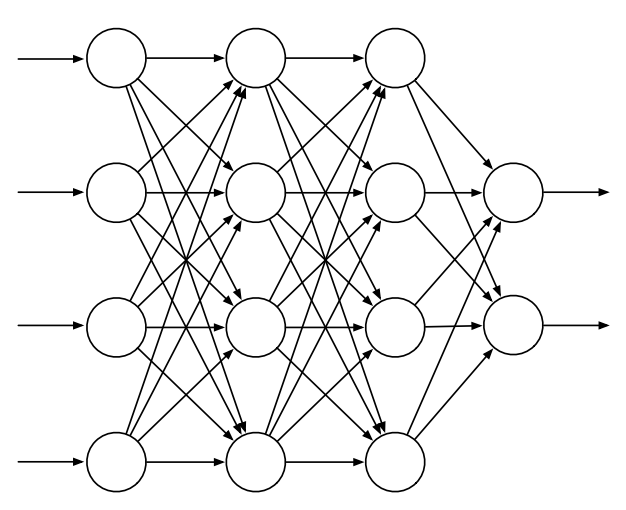
\includegraphics[scale=0.45]{figs/ann}
    \caption{A generic feedforward ANN with four input units, two output units, and two hidden layers}\textsuperscript{2}
    \label{fig:ann}
\end{figure}

Where we have some ability to optimize performance comes with the number of hidden layers we use, the size of the hidden layers, the optimizer function used, and the learning rate of this optimizer. While it would be valuable to measure our agents performance with hyperparameter tuning each of these, due to time and resource constraints, we explore only the hidden layer dimension as a hyperparameter later in this paper.

\section{Deep Q-Network (DQN)}
\begin{algorithm}
    \label{alg:1}
    \SetAlgoLined
    Init replay memory D to capacity N\;
    Init action-value function Q with random weights $\theta$\;
    Init target action-value function \^Q with weights $\theta$\textsuperscript{-} = $\theta$\;
    \For{episode = 1, 2000}{
    Init state\;
        \For{t = 1, 500}{
            With probability $\epsilon$ select random action a\textsubscript{t}
            Otherwise select a\textsubscript{t} = argmax\textsubscript{a}Q($\phi$(s\textsubscript{t}), a; $\theta$);
            Execute action a\textsubscript{t}, observe r\textsubscript{t} and next state s\textsubscript{t+1};

            Store transition (s\textsubscript{t}, a\textsubscript{t}, r\textsubscript{t}, s\textsubscript{t+1}, is\_terminal) in D

            Sample random minibatch of transitions from D
            \eIf{Every C steps}{
                \For{(s\textsubscript{t}, a\textsubscript{t}, r\textsubscript{t}, s\textsubscript{t+1}, is\_terminal) in minibatch}{
                    \eIf{is\_terminal}{
                        y\textsubscript{j} = r\textsubscript{t}
                    }{
                        y\textsubscript{j} = r\textsubscript{t} + gamma * max\textsubscript{a'}\^Q(s\textsubscript{j+1},a'; $\theta$)
                    }
                }
                Perform gradient descent step;\break
                Reset \^Q = Q;
            }{
                do nothing
            }
        }
    }
    \caption{deep Q-learning with experience replay}
\end{algorithm}

In algorithm \ref{alg:1} we see the full DQN algorithm, as implemented in project 2. This algorithm was implemented according to the DQN developed by DeepMind\textsuperscript{1}.

This algorithm has parts that look and feel much like the Q-learning we implemented in HW4. However, Q-learning has a tendency to become unstable when a nonline function approximator (such as neural network) is used to represent the action-value function. DeepMind addressed this with two novel approaches, which we have recreated in our own DQN. The first is to reduce correlations present in a sequence of observations by accumlating state/action/reward pairs over N number of steps across M number of epochs (capped at some arbitrary value) and storing them in a \textit{replay memory}. Then, uniformally selecting a random subset from the \textit{replay memory}, we apply a Q-learning off-policy weight update. Second, to avoid a tendency in the target-action-value \hat{Q} function to diverge, we periodically reset it to another action-value function \textit{Q}.

\section{Lunar Lander}
The Lunar Lander, developed by OpenAI Gym, is a RL environment in which the agent attempts to land a space craft on the moon. The state space includes 6 continuous variables, and two discrete: \textit{(x, y, x-velocity, y-velocity, angle, angle-velocity, left-leg, right-leg)}.

The first two variables, \textit{x} and \textit{y} are the horizontal and vertical coordinates of the space craft in the 2-dimensional map. The next two, \textit{x-velocity} and \textit{y-velocity} show the velocity with respect to the first two variables. \textit{angle} and \textit{angle-velocity} describe the upright angle of the space craft, and the velocity at which it is turning (positive value denotes clock-wise, negative denotes counter clock-wise). The last two discrete variables, \textit{left-leg} and \textit{right-leg} are boolean values indicating if the left/right leg are touching the ground or not.

The reward structure of this environment is as follows. The space craft receives between 100..140 points for moving from the top of the screen to the landing pad (ending with zero speed). If it moves away from the landing pad, it loses equivalent reward. The episode terminates when the lander either crashes or comes to a rest, receiving an additional -100 or +100 points. Each leg contact is +10 points. Finally, firing the main engine is -0.3 points each frame.

The action space consists of four discrete actions: do nothing, fire left orientation engine, fire main engine, fire right orientation engine.

\section{Training/Testing the Agent}
Graph: Reward at each training episode while training your agent and discussion of results
Graph: Reward per episode for 100 consecutive episodes using you trained agent and discussion of the results.

\section{The Effect of Epsilon-Decay on Policy Convergence}
Graphs

\section{The Effect of Gamma on Policy Convergence}
Graphs

\section{The Effect of CNN Hidden Layer Size on Policy Convergence}
Graphs

\section{Pitfalls \& Problems}
Explanation of pitfalls and problems you encountered.
Explanation of algorithms used: what worked best? what didn’t work?

\section{Further Research}
What would you try if you had more time?

\begin{thebibliography}{00}
\bibitem{b1} Volodymyr Mnih, Koray Kavukcuoglu, David Silver, Andrei A. Rusu, Joel Veness, Marc G. Bellemare, et al. (2015). Human-level control through deep reinforcement learning. Nature, p529-533. doi: 10.1038/nature14236
\bibitem{b2} https://gym.openai.com/envs/LunarLander-v2/
\end{thebibliography}

\end{document}
